\section{Visualizing the demographic spatio-temporal evolution}
Beyond the objective of allowing the study of inconsistent data, our method
includes incremental developments in most steps of the analysis, from data
representation to the visualization method for the clusters.
Figure~\ref{fig:overview} presents an overview of the processing steps of the
proposed method.



\begin{figure}
    \centering 
    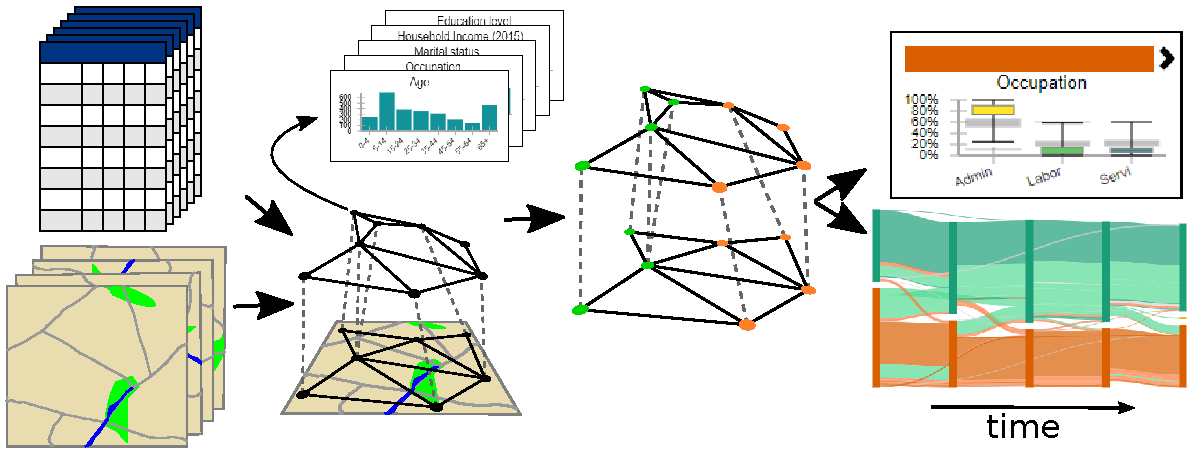
\includegraphics[width=0.975\linewidth]{overview.pdf}
    \caption{Overview of the proposed method. A graph is generated combining the
        original census data, encoding the changing geographical information.
        The graph is partitioned into an hierarchy~\cite{markus2017}. The
        characteristics and evolution of the clusters are then visually
        represented.
        \label{fig:overview}}
\end{figure}


\subsection{Census methodology and data representation}

Census data is disseminated in a tabulated form for aggregation areas: whole
country, state/province, metropolitan region, and so on. To provide as much
detail as possible, we focus on the smallest region with available data:
\emph{census tracts} (CT). They are usually defined to maintain the anonymity of
the population, leading to a population count in the order of thousands in
densely populated areas. Physical barriers are usually adopted as borders, so
these regions can change because of new roads, construction or removal of high
density buildings, and so on. Some census entities also consider demographic
characteristics, aiming to establish the CTs as a cohesive unit. Therefore, CTs
are the least geographically stable tabulation area.


Each CT is associated with a series of variables, with counts derived from the
census questionnaires, covering several aspects of the demographic
characteristics of the population. Some questions allow for multiple choices or
open answers, that are then tabulated into the most frequent categories. Since
the census is often used to direct government initiatives, which variables are
measured/disseminated is dependent on administrative interests, the general
understanding of the population, and current customs. For instance, income is
disseminated with a finer tabulation in the lower portion than on the higher. 


To match these variables over time and allow for direct comparison across
different census years, we aggregated similar ones (e.g. White, Black, Asian,
Other) into \emph{aspects} (e.g. Race), encoding the distribution of that facet
of the population. In this convention, we refer to the composing parts of an
aspect as a \emph{part} or the traditional \emph{variable}. Internally, the
aspects are represented using normalized histograms. This normalized
representation is crucial for the comparison between inconsistent regions.


In our graph based representation, each CT of each census year is represented as
a node, and edges are placed between nodes if the corresponding CTs share
geographic borders in the same year. Further, edges are placed between nodes if
the corresponding CTs belong to sequential years and there is geographical
overlap between them. This approach leads to a single graph representing the
whole spatio-temporal space of the data. Our objective then becomes to identify
partitions of this graph such that the nodes of each partition are more similar
between themselves than to the other nodes. This representation is not the only
option, nor unique, but it allows the use of existing graph-based methods for
the other steps.

\subsection{Geographic content clustering}
To partition the graph we must first establish a distance function between the
nodes, measuring the data similarity. This similarity is then associated with
the edges, leading to a weighted dynamic graph. Every node has a collection of
histograms, each representing the distribution of certain aspect in the
population.

Let $\G=(\V,\E)$ be a graph, where
$\V=\{\vertice_1,\vertice_2,\dots,\vertice_n\}$ is the set of nodes and
$\E=\{(\vertice_i,\vertice_j), i\not=j\text{ and }i,j \in [1,n]\}$ is the set of
edges. A function $\Hist$ associates each node to a set of $K$ histograms. We
define the distance $\D$ between two nodes $\vertice_i$ and $\vertice_j$ as:

\begin{equation}
    \D(\vertice_i,\vertice_j)=\sum_{k \in [1,K]}{\weight_k\, d(\Hist_k(\vertice_i),\Hist_k(\vertice_j))}
    \label{eq:dist}
\end{equation}

\noindent where $d$ is a distance metric between histograms and $\weight$ is a
sequence of non-negative weights associated with each aspect,
$\sum_{k\in[1,K]}{\weight_k}=1$. While any histogram metric can be used, we
adopted a euclidean distance between the vectors, because it led to reasonable
results with reduced computational cost. Therefore the distance between two
nodes is defined as the weighted average distance between its associated
histograms, where the weights can be adjusted by the user.

Once the distances are associated to the edges, we use watershed
cuts~\cite{Cousty2009} to create an initial clustering, which is then refined
into a hierarchy using the Sorted Maximal Matching (SMM)~\cite{markus2017} with
median linkage. The initial watershed step is performed to create an initial
clustering and reduce the running time of the SMM. For completeness, we briefly
review this method, but we refer the reader to the original
paper~\cite{markus2017} for more details, including a complete performance
evaluation using several metrics.


We included two application-specific parameters: the maximum number of clusters
to be shown and a distance threshold. Contrarily to the original SMM, which
merges all clusters in all steps, we only merge two clusters where the distance
is above the threshold after we reach the maximum number of displayed clusters.
Without this restriction, significantly different clusters would be merged
early, leading to increased intra cluster variance and the disappearance of
small outlier regions. Further, after the maximum number of clusters is reached,
we create one step of the hierarchy for each merge, leading to a binary
partition tree. In this structure we can directly access a result with an
arbitrary number of clusters.


Each resulting cluster is contiguous in the graph. This means that two similar,
but non-contiguous, sets of CTs will be classified into two different clusters,
which can be counterintuitive. To overcome this issue, we \emph{augment} the
graph with two new edges per node from a nearest neighbors
graph~\cite{scikit-learn} using only the distances between the histograms. These
edges connect nodes with similar content, if they are not already connected,
providing a path for the algorithm to group similar nodes. Theoretically, adding
more of these content based edges could be used to decrease the impact of the
spatio-temporal edges, controling the balance between content and topology in
the result. In practice, the effect is dependent on the data itself, and the
results are not consistent, or predictable, across different cities. We fixed it
at two edges because it was the lowest number that empircally led to consistent
clusters, but we believe that this idea warrants further investigation, as an
alternative to mixing parameters in the distance metric~\cite{Chavent2017}.



\subsection{Cluster characterization and variable relevance}
\label{sec:relevance}
The composition of each cluster is determined by simple statistical measures,
considering each aspect separately. We compute the minimum, maximum, median,
25\%, and 75\% quantiles for each part of each aspect for all clusters in the
hierarchy. While interpreting these values is more complex than interpreting
just the average, they provide far more information about the underlying
distribution.


We also use these statistical measurements to discover what characterizes each
cluster, that is, what makes it different from the others.  We define the
\emph{relevance} of a part of an aspect based on the distance between the
interquantile ranges (IQR) of the clusters in the same hierarchical level. If
the IQRs overlap for all clusters, that variable is not relevant to the
characterization of the cluster, but if the IQRs are distant, it means that this
specific range of values is something that only occurs in this cluster. 


\subsection{Clusters and trajectories}
While the partition of the data into different clusters helps the user to
understand what demographic groups exist and where they are, we are also
interested in the changes in those groups. To this end, we introduce the concept
of \emph{trajectories}, which are composed by regions that are classified into
the same sequence of clusters over the considered period. This enables direct
access to regions that evolved in the same manner. While the interface provides
access to data by census tract, the trajectories are the main unit of
exploration in this work.

\subsection{Colors}
\label{sec:colors}
As illustrated by Figure~\ref{fig:ui} and further explored in the next
subsection, our proposed interface heavily relies on color to express
cluster-related information. We adopted this convention because colors can be
used in all our visual tools in a coherent manner. However, this also introduced
significant challenges. The first is the limit on the number of clusters that
can be visually represented.  We limited the number of clusters to eight because
this was the largest number of colors that we could reliably use, derived from
the 8-class Dark2 set from ColorBrewer~\cite{ColorBrewer}. 

While we can reasonably limit the number of clusters, there are far more
possible trajectories. And the color associated with each trajectory should bear
some resemblance to the clusters included in it. Therefore, we were left with a
conundrum: \emph{Should we associate each trajectory with a unique color, which
the user probably cannot distinguish, or should we use a reduced set of colors
and associate the same color to different trajectories?} Since there are
advantages and disadvantages for each of those options, we adopted both. The
user can control which color policy is used via a checkbox in the configuration
panel, on the top left of the interface.

By default, the interface adopts a simplified color scheme, where a trajectory
is painted in the same color of a cluster if the regions were associated to that
cluster for \emph{all} times; in a slightly less saturated version of that color
if the regions were associated to that cluster for \emph{the simple majority} of
the time, and gray otherwise. In this mode, the colors will mostly represent
stability, immediately identifying the regions that were consistently associated
with each cluster. It also easily identifies volatile regions, painted gray.


When this simplified color scheme is disabled, each trajectory will be painted
using the average of the colors of the involved clusters, in the LAB color
space. In this mode, the map becomes more similar to a heatmap, where stronger
presence of a color indicates more temporal affinity to the cluster. Volatile
regions will also tend to be displayed in gray, as the average of three or more
colors.

\begin{figure}
    \centering 
    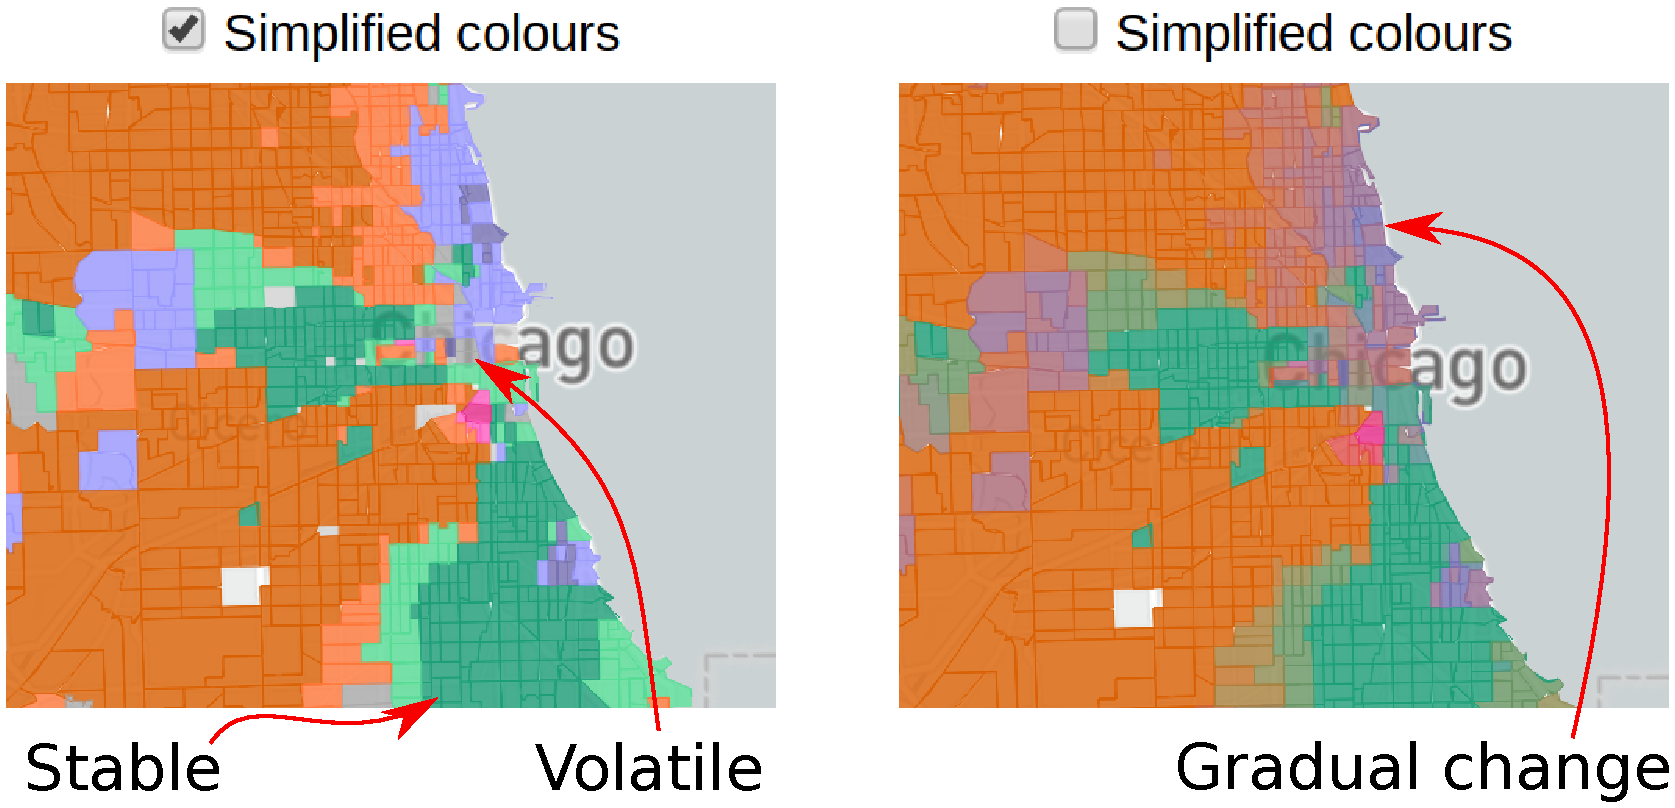
\includegraphics[width=0.95\linewidth]{colours.pdf}
    \caption{Different color schemes for Chicago with four clusters. Left:
    simplified, right: average color.\label{fig:colour}}
\end{figure}

While both approaches will use more than eight colors, in practice this is not
as significant because most cities can be explained using less than eight
clusters.  In fact, articles in the literature usually employ from two to five,
which are fairly stable across time. For the more dynamic scenarios, user
interaction can be used to alleviate the shortcomings of both approaches.


\subsection{User interface}
\label{sec:ui}
The initial interface is illustrated in Figure~\ref{fig:ui}. Since demographic
data can be nuanced, with intricate interconnections, we decided against
validating the interface using a synthetic dataset, considering instead data
from the Chicago region between 1970 and 2010, using previous published studies
as corroboration. This region is known for its entrenched racial divide and the
emergence of a \emph{'young urban'} population with a higher education
level~\cite{Delmelle2016,Delmelle2017}. More details about this dataset are
presented in Section~\ref{sec:study}, with an workflow example in
Figure~\ref{fig:chiWorkflow}.

\begin{figure*}
    \centering 
    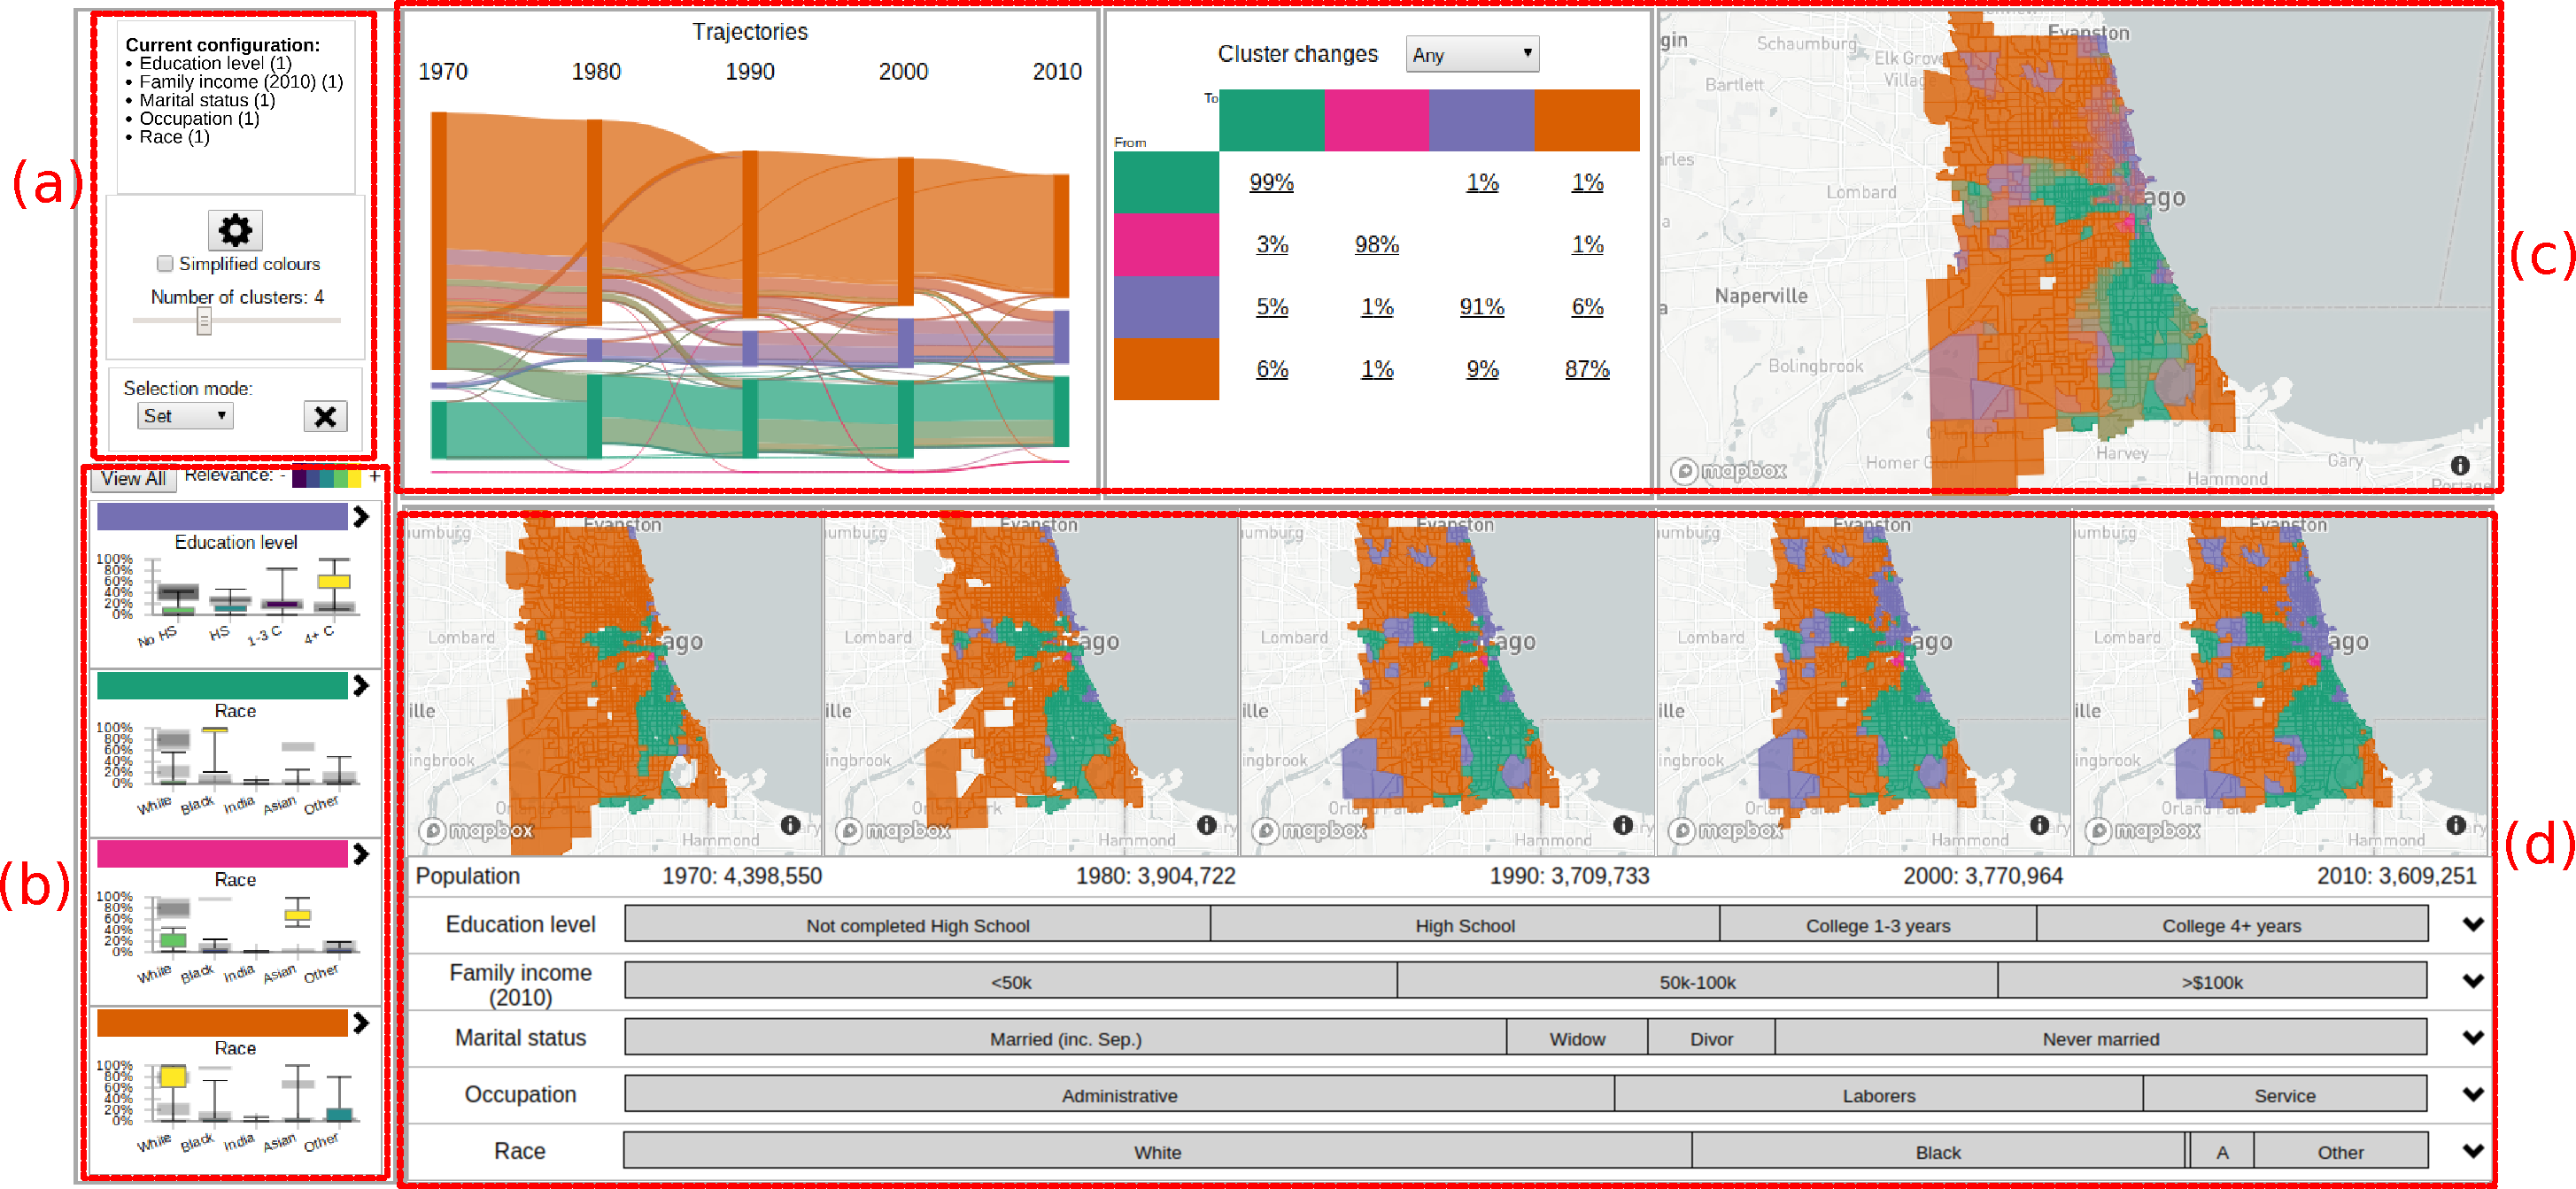
\includegraphics[width=0.95\linewidth]{ui.pdf}
    \caption{Initial interface of our method showing the demographic evolution of Chicago. 
        \textbf{(a)}: Configuration panel with the current clustering parameters and controls.
        \textbf{(b)}: Cluster overview illustrating the most relevant aspect for each cluster. 
        \textbf{(c)}: Trajectories overview and the general evolution of the population, geographical information, and how it changed. 
        \textbf{(d)}: Details of the selected trajectories, including precise geographic locations, population numbers, and the composition of the aspects.\label{fig:ui}}
\end{figure*}


The configuration panel, on top left in Figure~\ref{fig:ui}, displays which
aspects were used and their weights (following Equation~\ref{eq:dist}). It also
includes other configuration options that can be altered without re-processing
the data, such as the number of clusters and the color option. The gear button
allows access to the other configuration options that do require further
processing, such as changing location, aspects, and weights. This panel also
includes the configuration of the selection mode for the trajectories, which
allows the user to set, add, or remove the next selected trajectories to the
current selection. This feature enables the analysis of complex sets of
trajectories.


The cluster overview panel, on the bottom left in Figure~\ref{fig:ui}, displays
a brief summary of each cluster, based on the distance between the IQRs, as
detailed in Section~\ref{sec:relevance}. The \emph{View all} button opens a new
panel where all aspects are represented, while the chevron at the side of the
color lets the user expand each cluster separately. While the standard approach
to represent cluster characteristics is to use parallel
coordinates~\cite{johansson2005revealing,guo2006visualization}, this
representation occupies screen space proportional to the number of variables and
can get cluttered with a higher number of clusters, or when the clusters are not
well defined for multiple variables. To save space and leverage the familiarity
scientists have with statistical tools, we opted to use boxplots to properly
convey the distribution of each variable in the current cluster. However, a
simple boxplot would not include information about the other clusters, forcing
the user to mentally compare them to find what is relevant. 

We adopt an \emph{enhanced} version of the traditional boxplot, which includes
the minimum, maximum, 25\% and 75\% quantiles for the current cluster, but also
the IQRs for the other clusters, in slightly larger and faded black rectangles.
We also color the current IQR according to its relevance. While there might be
some degree of similarity between the color schema for relevance and for
trajectory identification, none of the experts consulted reported confusion.
Indeed, one expert reported confusion regarding the grey rectangles that
represent the IQRs for other distributions when they are not colored; when that
variable is not relevant to the characterization of the cluster. These simple
changes allow the user to easily understand the composition of the cluster and
how it relates to the others. Violin plots~\cite{hintze1998violin} could also be
used, providing more information about the shape of the distribution, but with
increased potential for obstructing the representation of the other clusters.


For instance, the boxplot that summarizes the purple cluster illustrated in
Figure~\ref{fig:ui}, detailed on Figure~\ref{fig:boxplot}, illustrates that this
cluster is best defined by the proportion of the population with four or more
years of college. The user can quickly see that this is relevant because the
corresponding IQR is colored with the highest relevance present in the legend.
It is also clear that, while this cluster includes CTs that have between 10\% to
90\% of people in this variable, approximately, half of them have about 60\% of
the population with four or more years of college. Since all the other IQRs are
well separated, this is a defining characteristic of this cluster. Conversely,
the proportion of the population with one to three years of college is not
relevant, as indicated by black fill in the rectangle representing the IQR of
this cluster, in overlapping position with the rectangles of the other clusters.
By clicking on the colored bar above the boxplot, the user can select all
trajectories that contain this cluster at any point in time.

\begin{figure}
    \centering 
    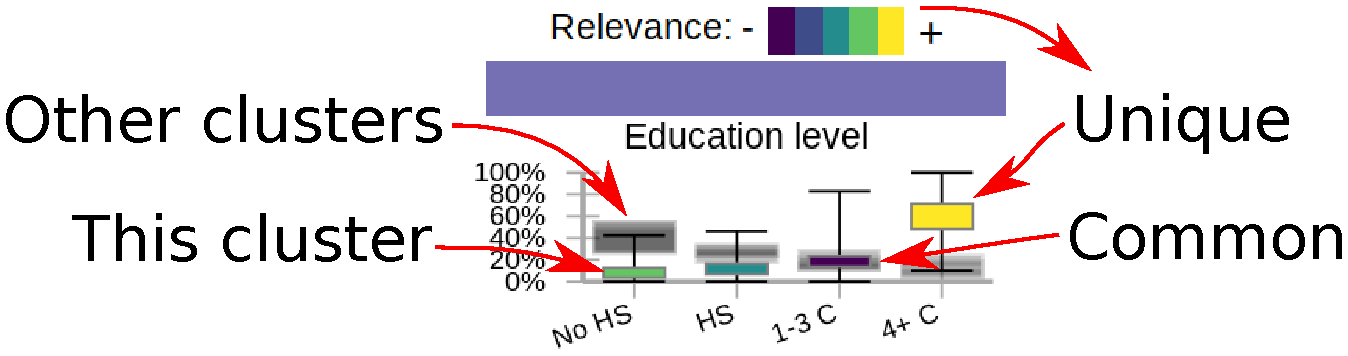
\includegraphics[width=0.9\linewidth]{boxplot.pdf}
    \caption{Enhanced boxplot of the clusters' characteristics allows a quick
    comparison to the other clusters.\label{fig:boxplot}}
\end{figure}


The other clusters identified on Figure~\ref{fig:ui} correspond to higher
concentration of people that identify as Black in the green cluster, people that
identify as "Asian, Hawaiian, other pacific islander" in the pink cluster, and
people that identify as White in the orange cluster. From these plots, it is
clear that the city is indeed racially divided~\cite{Delmelle2016}, with several
CTs that are almost exclusively occupied by people of the same racial category.


The trajectories overview aims to convey basic information about the
trajectories present in the data, where they are, and what changes are involved.
This is done using three sub panels. The first, on the left, contains a Sankey
diagram illustrating the evolution of the clusters over time. The widths are
proportional to the population involved, the colors follow a policy detailed in
Section~\ref{sec:colors}. A stacked graph could also be used to represent the
proportions of each cluster~\cite{Valdivia2015} with less clutter, since the
transitions between clusters would not be represented. However, this is only
viable if more temporal steps are available, making the plot smoother. Another
option to remove clutter is to remove portions of this plot when trajectories
are selected, but this would change the layout and compromise the user's mental
map.


In our example in Figure~\ref{fig:ui}, we can see that the total population of
Chicago is decreasing. Additionally, the orange and green clusters contain most
of the population and are fairly stable over time. The pink cluster is small and
mostly stable. The purple cluster is increasing, mostly by incorporating areas
that were previously orange. Since the purple group corresponds to the emergent
'young urban' group, this corroborates the findings of
Delmelle~\cite{Delmelle2016,Delmelle2017}. This diagram can also be used to
select specific trajectories, by clicking on the bands, or all trajectories that
contain a specific cluster at a specific time, by clicking on the rectangles.


The next sub panel, in the top middle of Figure~\ref{fig:ui}, is a transition
matrix between the clusters. It indicates the percentage of the population whose
area changed in each pattern. This kind of table can be found in the related
literature~\cite{Delmelle2016}, so it is familiar to the advanced users, and it
not only informs the proportional changes, but allows the selection of the
corresponding trajectories for further analysis.

Contrary to the trajectories plot, this representation is more Markovian, where
only the current and next state are considered. This panel also enables easier
access to trajectories with specific changes, by clicking on the corresponding
percentage values. The combo box allows the user to refine the transitions, from
'Any', which includes all transitions between years, to specific transitions, to
changes from the first year to the last year. In this example, approximately
99\% of the population in areas classified as green were also in areas
classified as green in the next year, while 1\% changed to purple at some point
and another 1\% to orange. The total is over 100\% due to rounding errors.
Regions changed from the orange to the green cluster for 6\% of its population,
1\% to pink, and 9\% to purple. This further corroborates the fact that most of
the growth of the purple cluster came from the orange cluster. Additionally, the
lack of transitions is also relevant, for instance, no CT changed from majority
of Black population (green) to Asian population (pink), and no CT with
significant Asian population had significant increase in education levels
(purple).

The panel in the top right of Figure~\ref{fig:ui} is a map of the region under
analysis, summarizing the geographical evolution of the clusters over time.  The
colors are derived from the clusters involved in each trajectory as detailed in
Section~\ref{sec:colors}, which are consistent across the linked views. 

The bottom part of the interface contains the details for the selected
trajectories, or for the whole city if nothing is selected, as illustrated in
Figure~\ref{fig:ui}. This panel contains two main regions: the small multiple
maps, depicting the clusters at each year, and the stacked bar plots that
summarize the overall composition of these regions. Some finer localization
information is lost using small multiples, such as small border changes, but
that information is available at the larger map. All the maps are linked with
syncronized navigation, and the use of small multiples allows the exploration of
each temporal census individually, and its comparison to the others, with
minimal interaction. 

In this example, the maps show the transition from orange to green and purple in
several regions over time. Clicking on a region in these maps will bring up a
new panel with the original census data of this specific region. The actual
population numbers are below the maps, and they confirm the notion provided by
the Sankey diagram that the total population is indeed decreasing. 

Each aspect is represented by a stacked bar plot, where the width of each
rectangle corresponds to the average percentage of that variable over the
considered period. We chose stacked bar plots to represent the composition of
the regions because they can accurately and succinctly inform the proportions of
each aspect, without any interaction. In this case, about half of the people in
Chicago in the considered period are married, and the percentage that are
Widowers or Divorced is roughly similar. About half of the population work in
Administrative jobs, a third never completed high-school, approximately half
have gross family income below 50,000USD per year. The vast majority identify as
white. Placing the mouse over one of the bars will open a small panel with the
temporal evolution of that specific variable, and clicking on the chevron on the
right side expands the corresponding aspect, showing details of the temporal
evolution of each variable and also the corresponding IQRs for the whole city.